\documentclass[11pt,oneside,a4paper,notitlepage]{article}
\usepackage{graphicx,amsmath,hyperref}
\usepackage[margin=2cm]{geometry}
\hypersetup{
    colorlinks=true, %set true if you want colored links
    linktoc=all,     %set to all if you want both sections and subsections linked
    linkcolor=blue,  %choose some color if you want links to stand out
}

\begin{document}
\tableofcontents

\part{Profiles NF2008}

\section{Normalized poloidal magnetic flux $\psi_N$}
Normalized polidal magnetic flux $\psi_N$ (\ref{eq:psi}, Fig.\ref{fig:Flux}):
\begin{equation}\label{eq:psi}
 \psi_N(a_N)=\dfrac{\int\limits_0^{a_N} \mu(a')a'da'}{\int\limits_0^{1} \mu(a')a'da'}
\end{equation}
where $\mu=1/q$, $q(a_N)=1+3.6a_N^{5.6}$ is safety factor.
\begin{figure}[h] 
 \centering
 \includegraphics[width=0.5\textwidth]{Flux.eps}
 \caption{$\psi_N$ - normalized poloidal magnetic flux (NF2008)} 
 \label{fig:Flux}
\end{figure}
\section{Density $n_e$ and temperature $T_{e,i}$}
Profiles of electron density $n_e(\psi_N)$ and electron and ion temperature $T_{e,i}(\psi_N)$ 
(\ref{eq:ne},\ref{eq:T}):
\begin{equation}\label{eq:ne}
 n_e(\psi_N)=n_{sep}+a_{n0}\Bigg[tanh\Bigg(2\frac{1-\psi_{mod}}{\Delta}\Bigg)-\\
 tanh\Bigg(2\frac{\psi_N-\psi_{mod}}{\Delta}\Bigg)\Bigg] \\
 +a_{n1}H\Bigg(1-\frac{\psi_N}{\psi_{ped}}\Bigg)\Bigg[1-\\
 (\frac{\psi_N}{\psi_{ped}})^{\alpha_{n1}}\Bigg]^{\alpha_{n2}},
\end{equation}
\begin{equation}\label{eq:T}
 T_{e,i}(\psi_N)=T_{sep}+a_{T0}\Bigg[tanh\Bigg(2\frac{1-\psi_{mod}}{\Delta}\Bigg)-\\
 tanh\Bigg(2\frac{\psi_N-\psi_{mod}}{\Delta}\Bigg)\Bigg] \\
 +a_{T1}H\Bigg(1-\frac{\psi_N}{\psi_{ped}}\Bigg)\Bigg[1-\\
 (\frac{\psi_N}{\psi_{ped}})^{\alpha_{T1}}\Bigg]^{\alpha_{T2}},
\end{equation}
where $\Delta$ is pedestal width, $\psi_{ped}=1-\Delta,\psi_{mid}=1-\Delta/2$, 
parameters $a_{n0},a_{t0}$ and $\Delta$ affect the pedestal profiles, 
parameters $a_{n1},a_{T1},\alpha_{n1},\alpha_{n2},\alpha_{T1}$ and $\alpha_{T2}$ affect the 
core plasma profiles, $H(x)$ - Heaviside function. These profiles are shown as function of 
normalized radius at Fig.\ref{fig:ne} and Fig.\ref{fig:T}.
\begin{figure}[h]
\begin{center}
\begin{minipage}[h]{0.4\linewidth} 
 \centering
 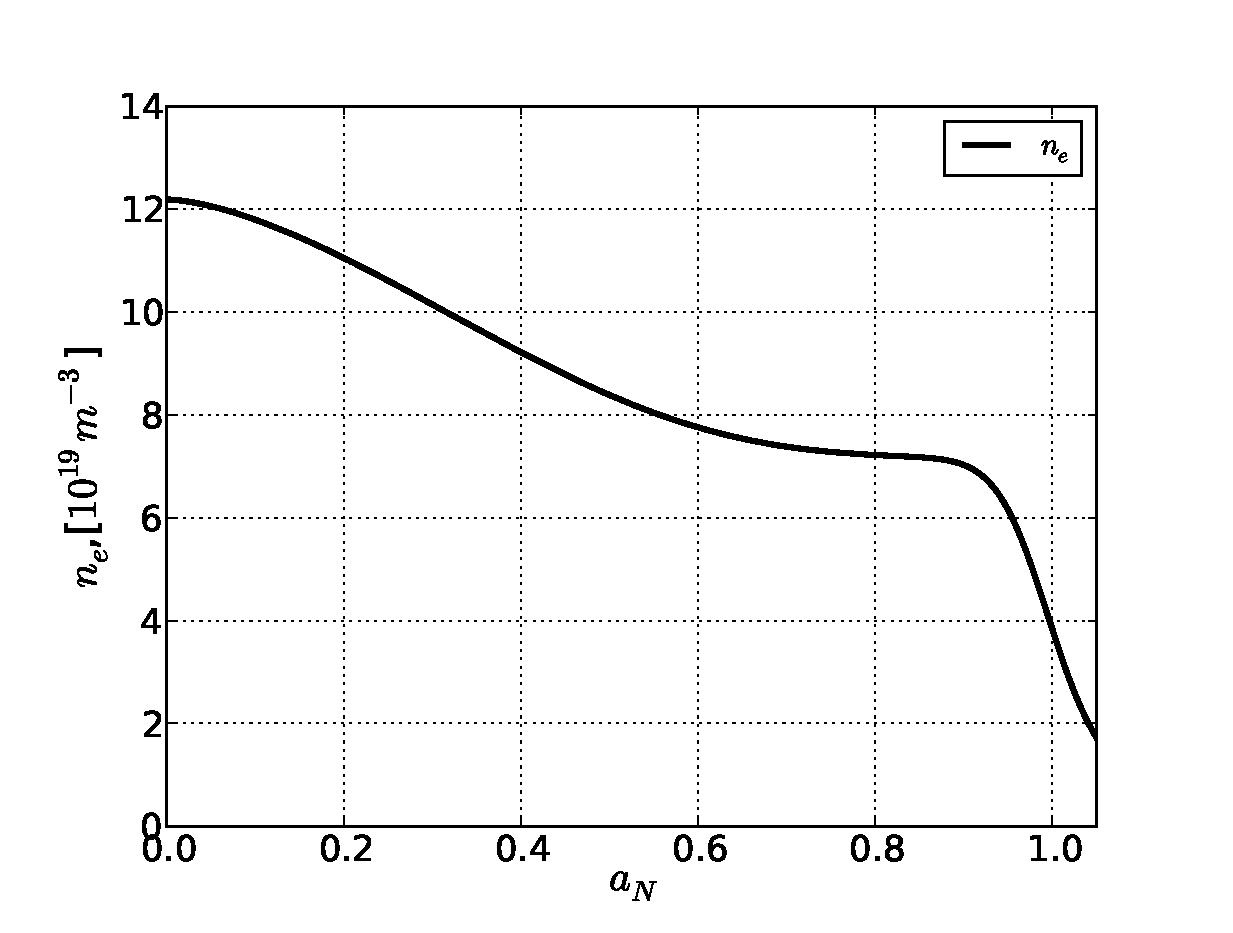
\includegraphics[width=1.35\linewidth]{ne.eps}
 \caption{Electron density, $10^{19} m^{-3}$ (NF2008)}
 \label{fig:ne}
\end{minipage}
\hfill
\begin{minipage}[h]{0.4\linewidth}
 \centering
 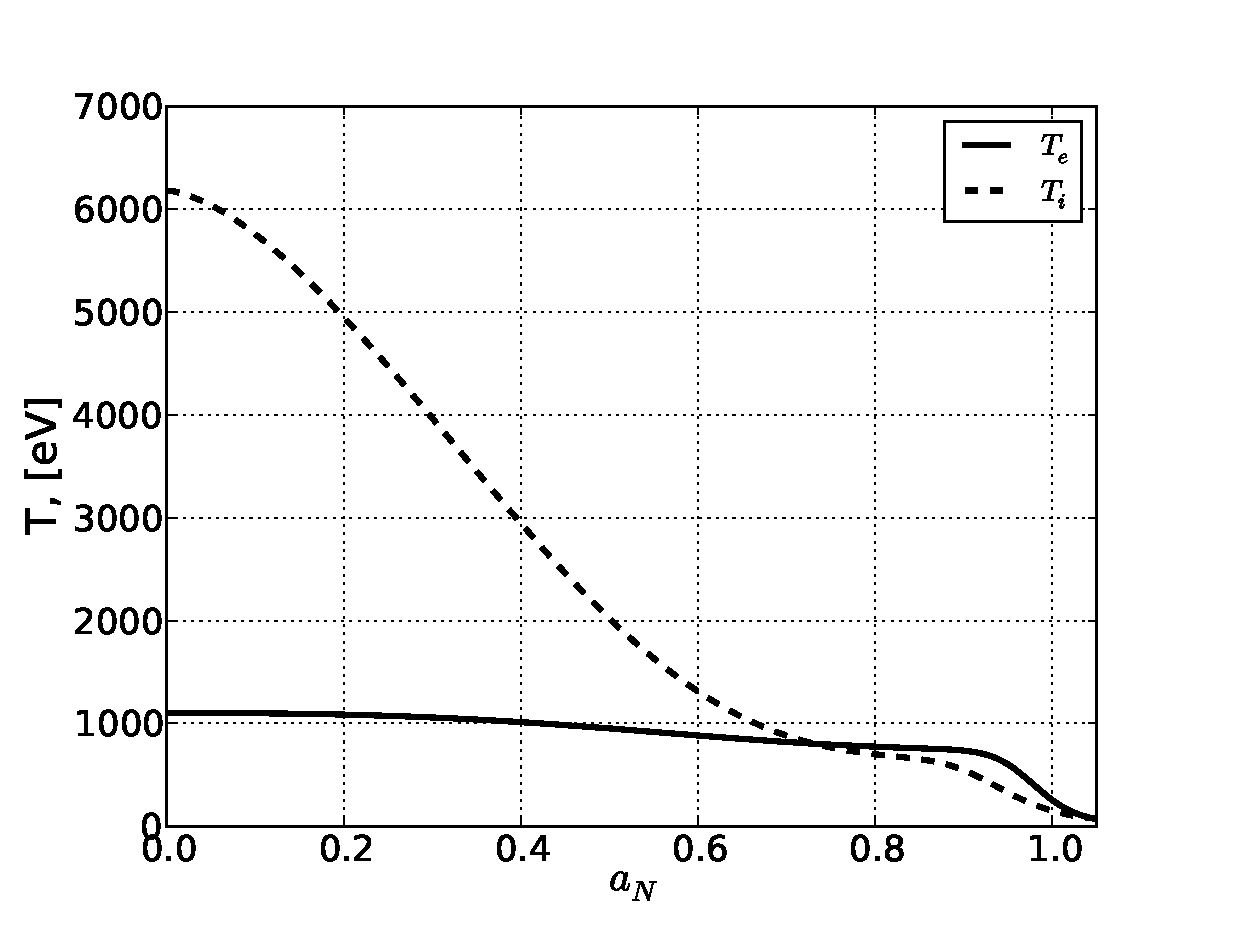
\includegraphics[width=1.35\linewidth]{T.eps}
 \caption{Electron and ion temperature, eV (NF2008)}
 \label{fig:T}
\end{minipage}
\end{center}
\end{figure}
\section{Plasma pressure and pressure gradients}
Electron, ion and total plasma pressure (Fig.\ref{fig:P}) are estimated as (\ref{eq:P}):
\begin{equation}\label{eq:P}
 P_{e,i}[Pa]=1.6\times n_e [10^{19}m^{-3}] \times T_{e,i}[eV]
\end{equation}
Pressure gradients are shown at Fig.\ref{fig:DP}.
\begin{figure}[h]
\begin{center}
\begin{minipage}[ht]{0.4\linewidth} 
 \centering
 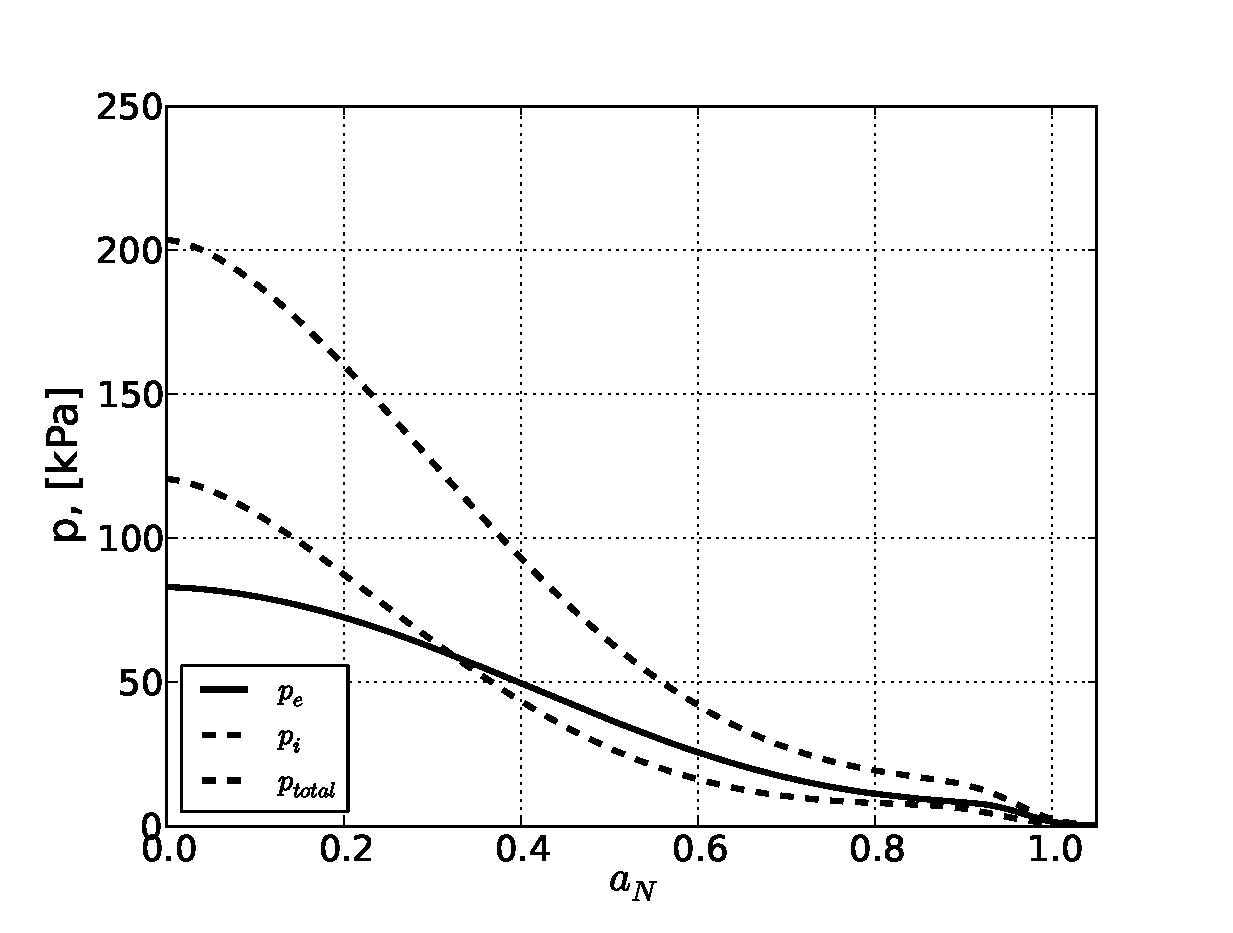
\includegraphics[width=1.35\linewidth]{P.eps}
 \caption{Electron, ion and total pressure, $kPa$ (NF2008)}
 \label{fig:P}
\end{minipage}
\hfill
\begin{minipage}[ht]{0.4\linewidth} 
 \centering
 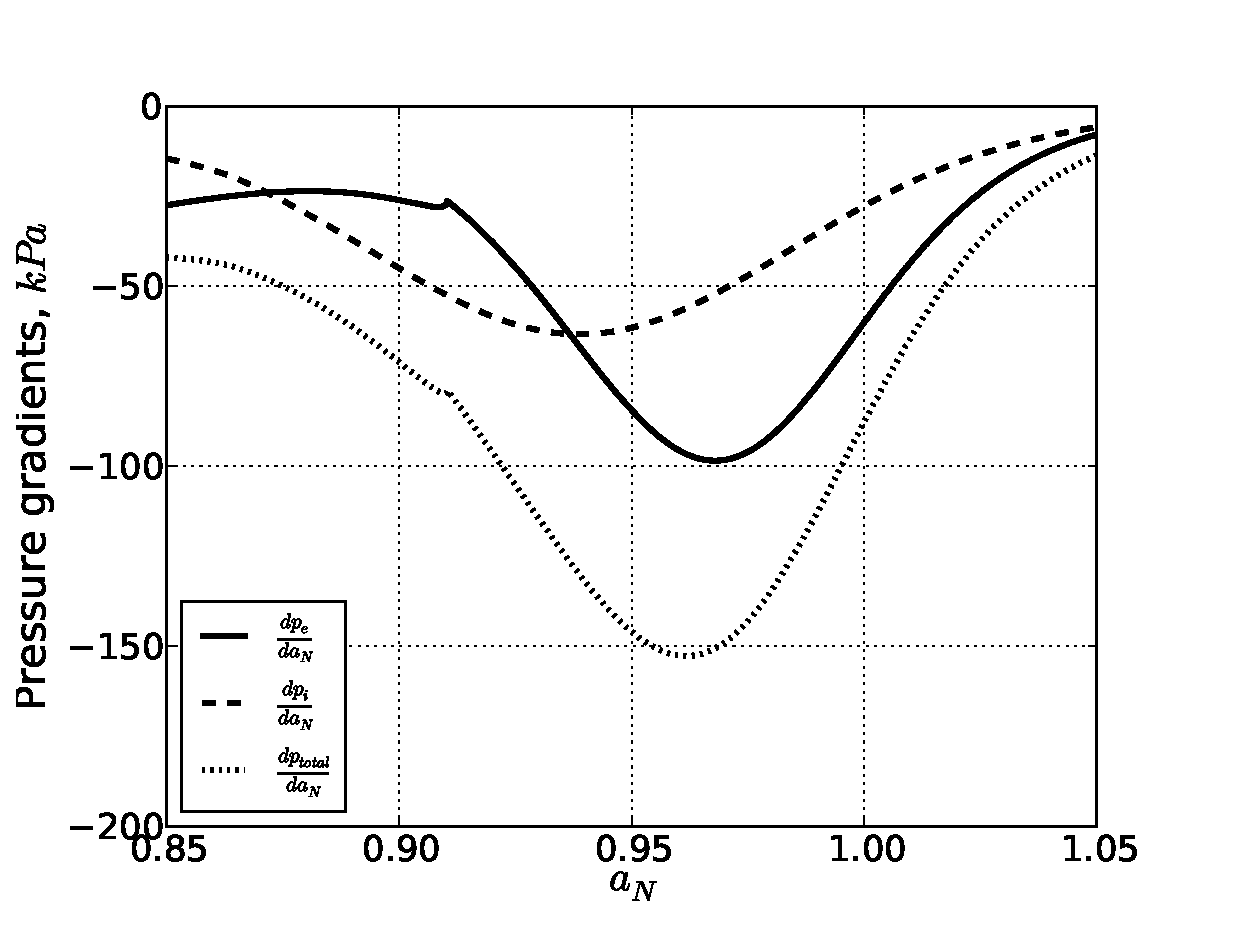
\includegraphics[width=1.35\linewidth]{DP.eps}
 \caption{Pressure gradients, $kPa$ (NF2008)}
 \label{fig:DP}
\end{minipage}
\end{center}
\end{figure}
\section{Radial electric field $E_{0r}(a_N)$}
Radial electric field $E_{0r}(a_N)$ (Fig.\ref{fig:Efield}) is aproximated as (\ref{eq:Efield}):
\begin{equation}\label{eq:Efield}
 E_{0r}(a_N)=d_1+r_1a_N\,exp\Bigg(b_1+c_1a_N^{exp(-a_1x^2)}\Bigg)[\frac{V}{m}]. 
\end{equation}
\begin{figure}[h]
\begin{center}
\begin{minipage}[ht]{0.4\linewidth} 
 \centering
 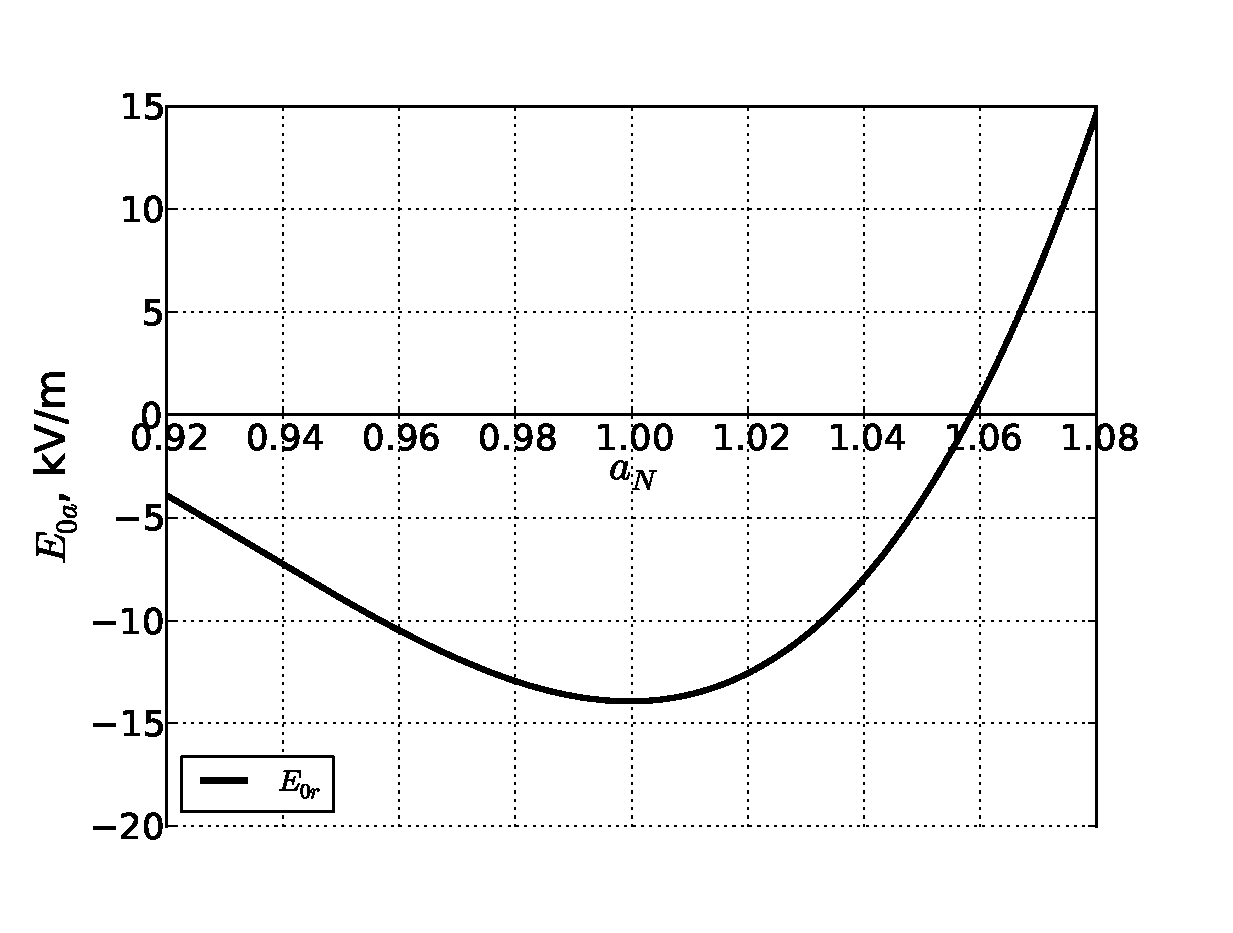
\includegraphics[width=1.35\linewidth]{E.eps}
 \caption{Radial electric field, $kV$ (NF2008)}
 \label{fig:Efield}
\end{minipage}
\hfill
\begin{minipage}[h]{0.4\linewidth}
 \centering
 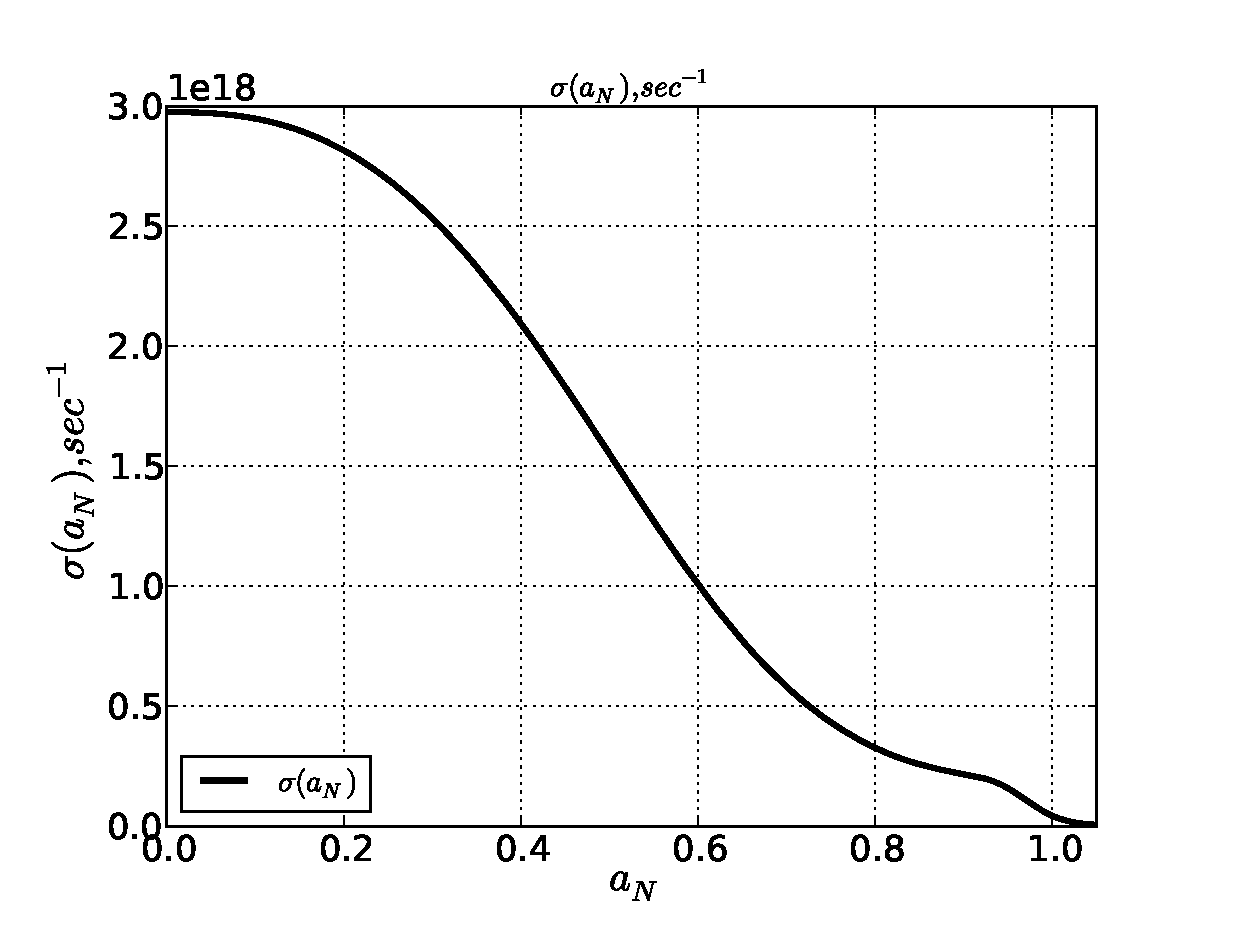
\includegraphics[width=1.35\linewidth]{sigma.eps}
 \caption{Plasma conductivity, $sec^{-1}$ (NF2008)}
 \label{fig:sigma}
\end{minipage}
\end{center}
\end{figure}
\section{Plasma conductivity $\sigma(a_N)$}
Plasma conductivity $\sigma(a_N)$ (\ref{fig:sigma}, Fig.\ref{fig:sigma}):
\begin{equation}
 \sigma(a_N)[sec^{-1}]=1.2\times10^{17}\Bigg(\dfrac{T_e[keV]}{500}\Bigg)^{3/2}
\end{equation}

\section{Equation}
Our equation (\ref{eq:equation:1}):
\begin{equation} \label{eq:equation:1}
\frac{1}{a_N}\frac{d}{da_N}\Bigg( a_N \frac{d}{da_N}(a_NB_m^a) \Bigg) \\
-\frac{m^2}{a_N^2}(a_NB_m^a)-\frac{m}{a_N^2}Q_m(a_N)(a_NB_m^a)- \\
\frac{4\pi m^2}{cB_{0\zeta}}\frac{R}{a}\frac{dj_b}{da_N}Q_{1m}(a_N)(a_NB_m^a)=0
\end{equation}
\section{$K_m(a_N), A(a_N)$}
Quantities $K_m(a_N)$ (Eq.\ref{eq:km}, Fig.\ref{fig:km}) and $A(a_N)$ 
(Eq.\ref{eq:km}, Fig.\ref{fig:A}):
\begin{equation}\label{eq:km}
 K_m(a_N)=F_m(a_N)\frac{a}{R}\frac{V_{0||}}{mc}+\frac{1}{B_0} \\
 \Bigg( \frac{1}{p_{0i}} \frac{dp_{0i}}{da_N} \frac{T_i(a_N)}{ea_{pl}}-E_{0a}(a_N) \Bigg)
\end{equation}
\begin{equation}
 A(a_N)=\frac{8\pi}{B_{0\zeta}^2}a_N \frac{dp_0}{da_N}m^2 (\mu^2-1- \\
 \frac{R}{a}S\xi'), ~~\fbox{$-1-\frac{R}{a}S\xi'\approx-9$}
\end{equation}
\begin{figure}[h]
\begin{center}
 \begin{minipage}[h]{0.4\linewidth}
  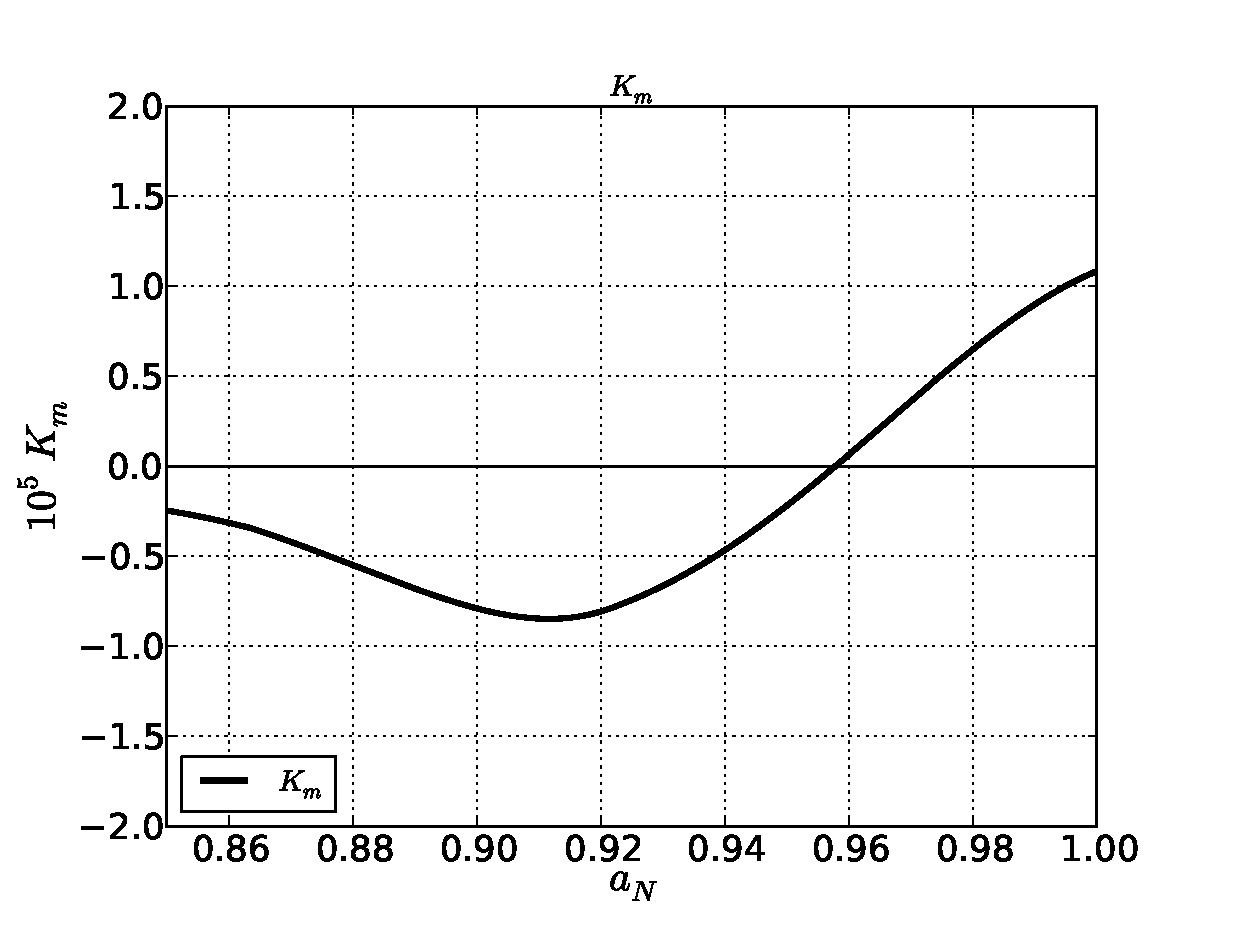
\includegraphics[width=1.35\linewidth]{Km.eps}
  \caption{$K_m(a_N)$ (NF2008)}
  \label{fig:km}
 \end{minipage}
 \hfill
 \begin{minipage}[h]{0.4\linewidth}
  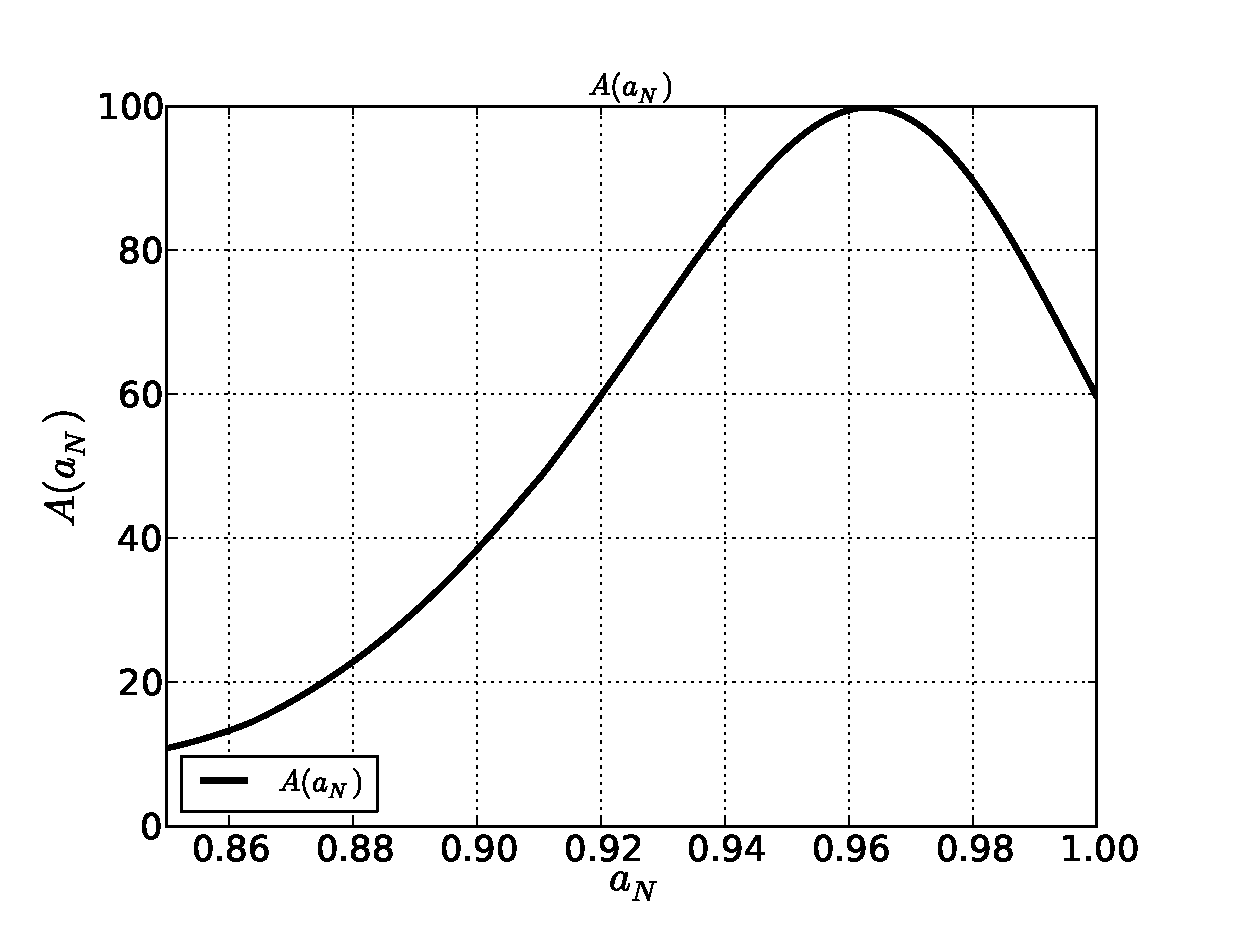
\includegraphics[width=1.35\linewidth]{A.eps}
  \caption{$A(a_N)$ (NF2008)}
  \label{fig:A}
 \end{minipage}  
\end{center}
\end{figure}
\section{$Q_m(a_N)$}
Real (\ref{eq:Q:r}) and imaginary (\ref{eq:Q:i}) part of $Q_m(a_N)$ (Fig.\ref{fig:Q}):
\begin{equation}\label{eq:Q:r}
 \textnormal{Re}Q_m=\frac{mK_m^2(a_N)F_m^2(a_N)A(a_N)}{\\
 \Bigg(mK_m(a_N)F_m^2(a_N)\Bigg)^2+\Bigg(A_m(a_N)\dfrac{c}{4\pi\sigma(a_N)a}\Bigg)^2}
\end{equation}
\begin{equation}\label{eq:Q:i}
 \textnormal{Im}Q_m=\frac{K_m(a_N)A^2(a_N)\dfrac{c}{4\pi\sigma(a_N)a} }{\\
 \Bigg(mK_m(a_N)F_m^2(a_N)\Bigg)^2+\Bigg(A_m(a_N)\dfrac{c}{4\pi\sigma(a_N)a}\Bigg)^2}
\end{equation}
\begin{figure}[h]
\begin{center}
\begin{minipage}[h]{0.4\linewidth}
 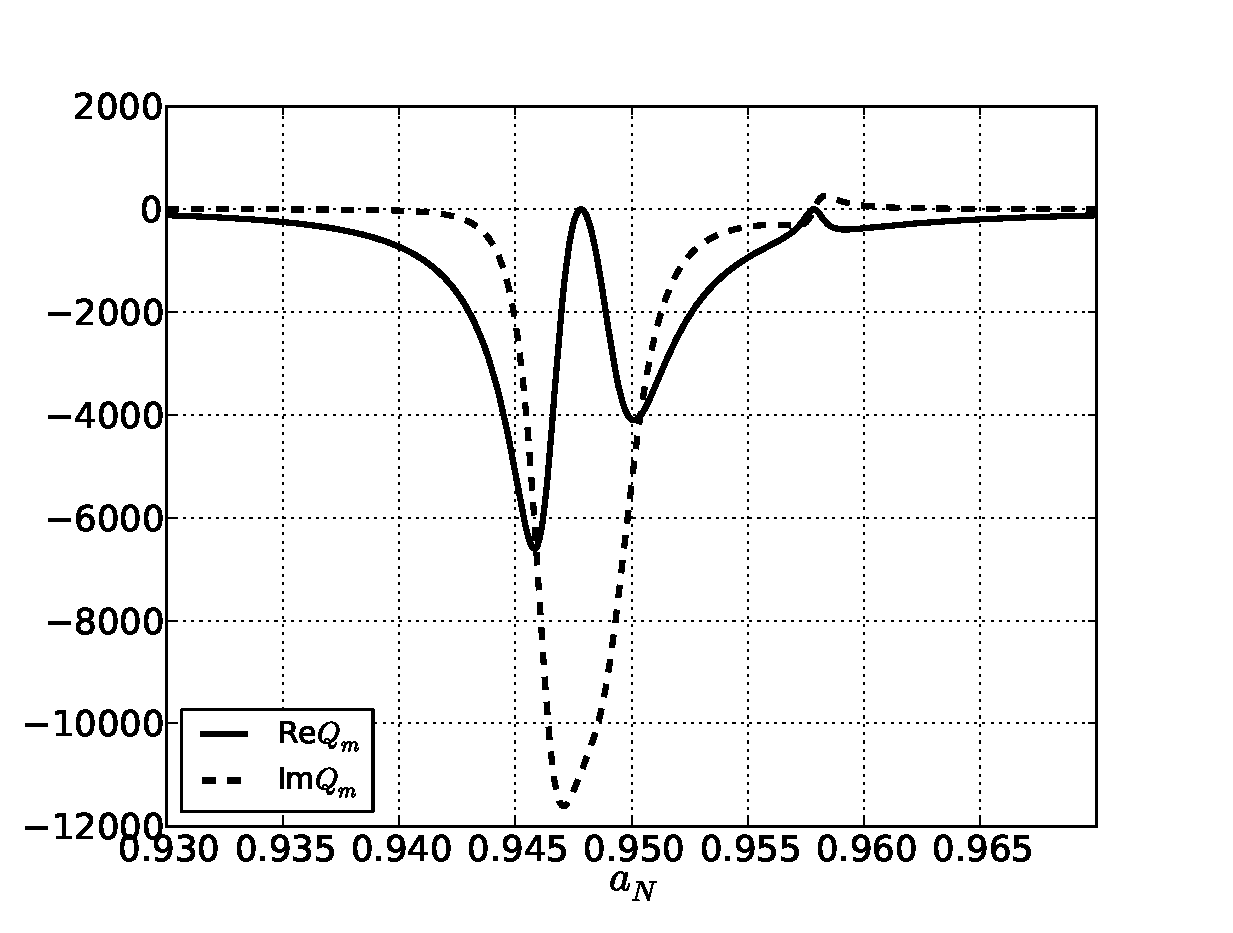
\includegraphics[width=1.35\linewidth]{Q.eps}
 \caption{$Q(a_N):~m=-11,V_{0}=0km/sec$ (NF2008)}
 \label{fig:Q}
\end{minipage}
\hfill
\begin{minipage}[h]{0.4\linewidth}
 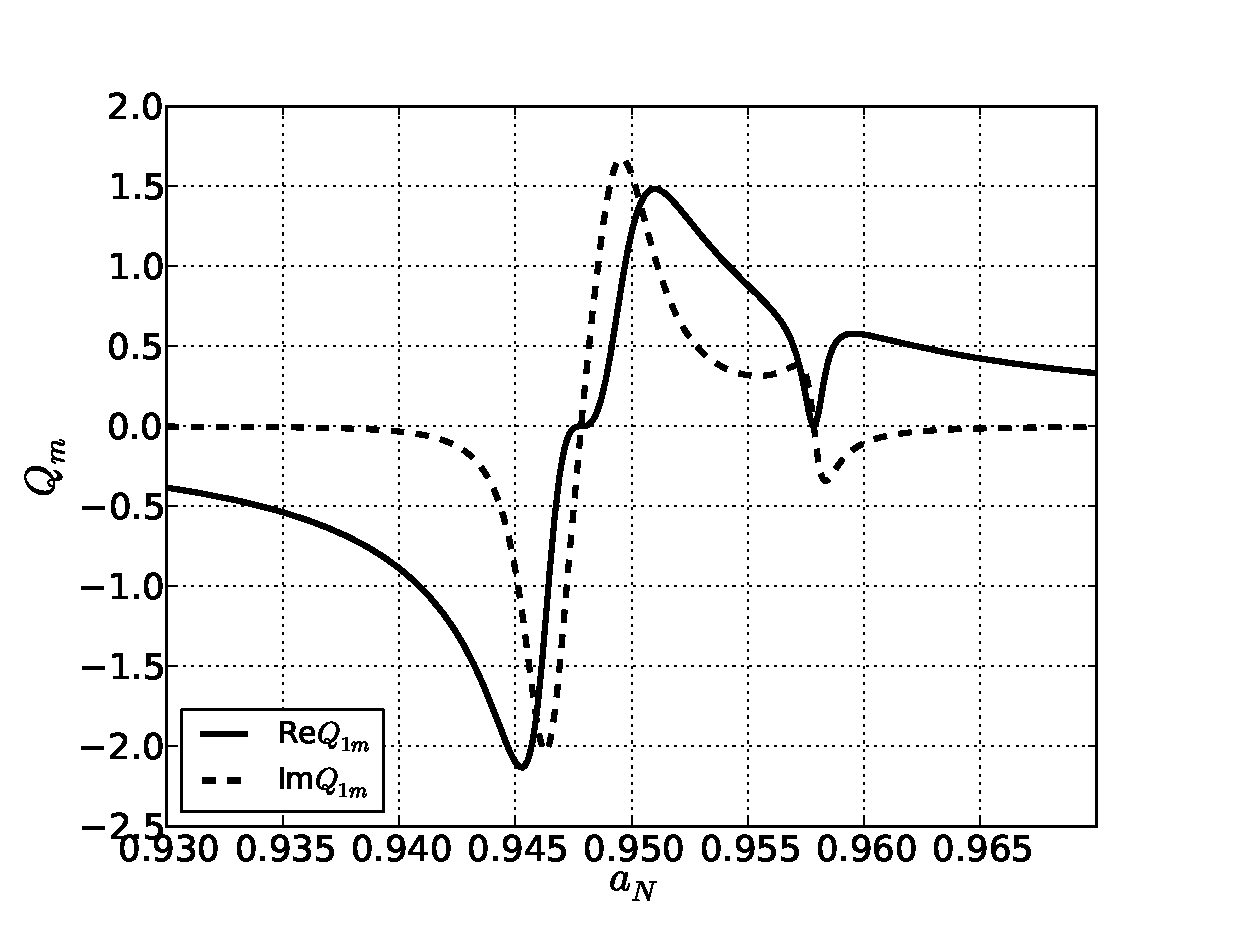
\includegraphics[width=1.35\linewidth]{Q1.eps}
 \caption{$Q_{1m}:~m=-11,V_{0}=0km/sec$ (NF2008)}
 \label{fig:Q1}
\end{minipage}
\end{center}
\end{figure}
\section{$Q_{1m}(a_N)$}
Real (\ref{eq:Q1:r}) and imaginary (\ref{eq:Q1:i}) part of $Q_{1m}$ (Fig.\ref{fig:Q1}):
\begin{equation}\label{eq:Q1:r}
 \textnormal{Re}Q_{1m}=\frac{mK_m^2(a_N)F_m^3(a_N)}{\\
 \Bigg(mK_m(a_N)F_m^2(a_N)\Bigg)^2+\Bigg(A_m(a_N)\dfrac{c}{4\pi\sigma(a_N)a}\Bigg)^2}
\end{equation}
\begin{equation}\label{eq:Q1:i}
 \textnormal{Im}Q_{1m}=\frac{K_m(a_N)F_m(a_N)A(a_N)\dfrac{c}{4\pi\sigma(a_N) a}}{\\
 \Bigg(mK_m(a_N)F_m^2(a_N)\Bigg)^2+\Bigg(A_m(a_N)\dfrac{c}{4\pi\sigma(a_N)a}\Bigg)^2}
\end{equation}
\section{Pressure perturbation $P_m$}
Real and imaginary part of pressure perturbations (\ref{eq:rpert},\ref{eq:ipert}):
\begin{equation} \label{eq:rpert}
 \textnormal{Re}P_m=-a_N\frac{dp_0}{da_N}\frac{R}{a} \\
 \frac{mK_m(a_N)F_m(a_N)A(a_N)\dfrac{c}{4\pi\sigma(a_N)a}}{\Bigg( \\
 mK_m(a_N)F_m^2(a_N) \Bigg)^2 + \Bigg( \\
 A(a_N) \dfrac{c}{4\pi\sigma(a_N)a} \Bigg)^2}\\
 \frac{B_m^a}{B_0}
\end{equation}
\begin{equation} \label{eq:ipert}
 \textnormal{Im}P_m=a_N\frac{dp_0}{da_N}\frac{R}{a} \\
 \frac{m^2K_m^2(a_N)F_m^3(a_N)\dfrac{B_{0\varsigma}}{B_0}}{\Bigg( \\
 mK_m(a_N)F_m^2(a_N) \Bigg)^2 + \Bigg( \\
 A(a_N) \dfrac{c}{4\pi\sigma(a_N)a} \Bigg)^2}\frac{B_m^a}{B_0}
\end{equation}
\begin{figure}
 \centering
 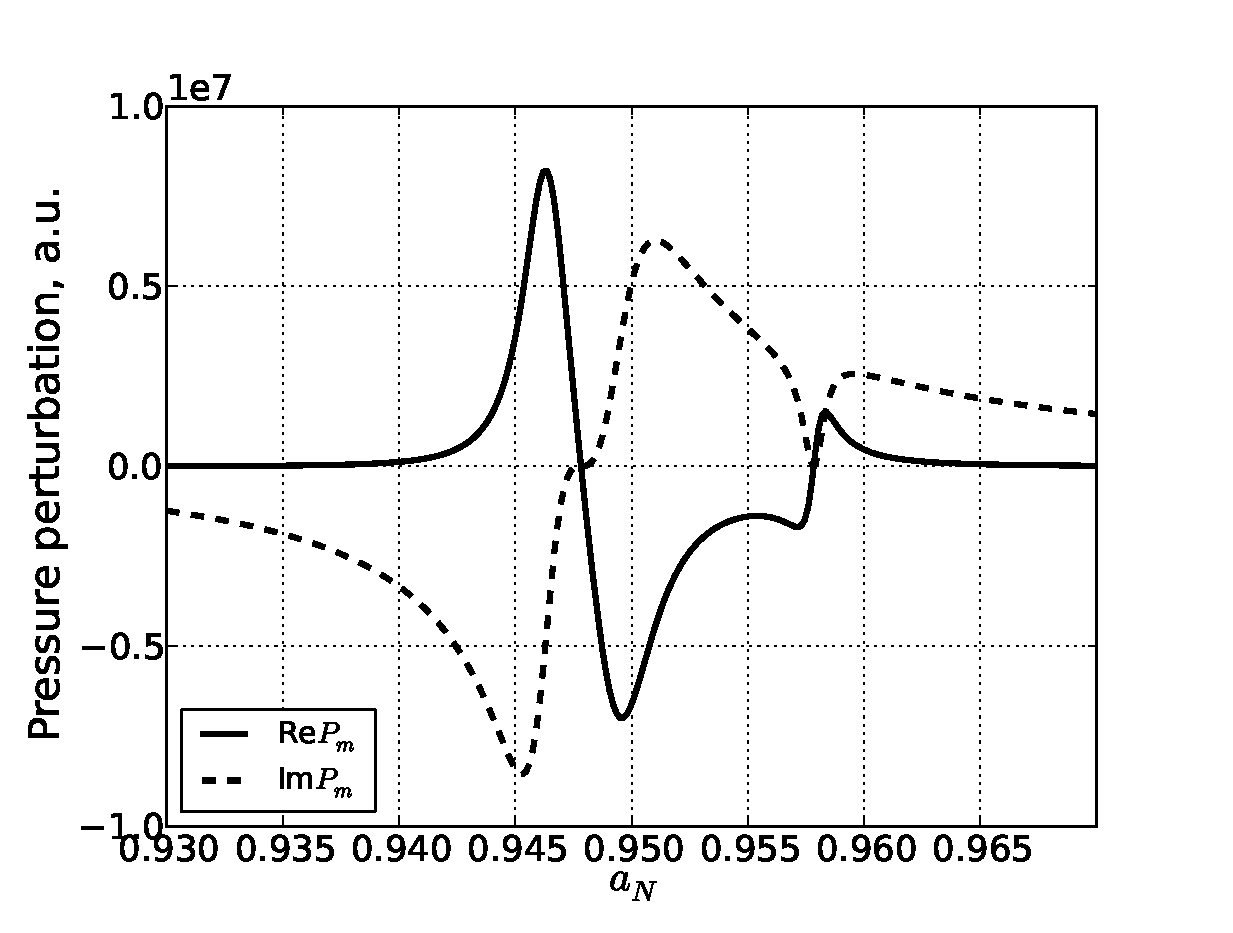
\includegraphics[width=0.7\textwidth]{perturbation.eps}
 \caption{Plasma pressure perturbation (NF2008)}
 \label{fig:pert}
\end{figure}



\newpage
\part{Profiles NF2013}
\section{Density $n_e$ and temperature $T_{e,i}$}
All subsequent profiles correspond $60^o$ phase.
\begin{figure}[h]
\begin{center}
\begin{minipage}[h]{0.4\linewidth} 
 \centering
 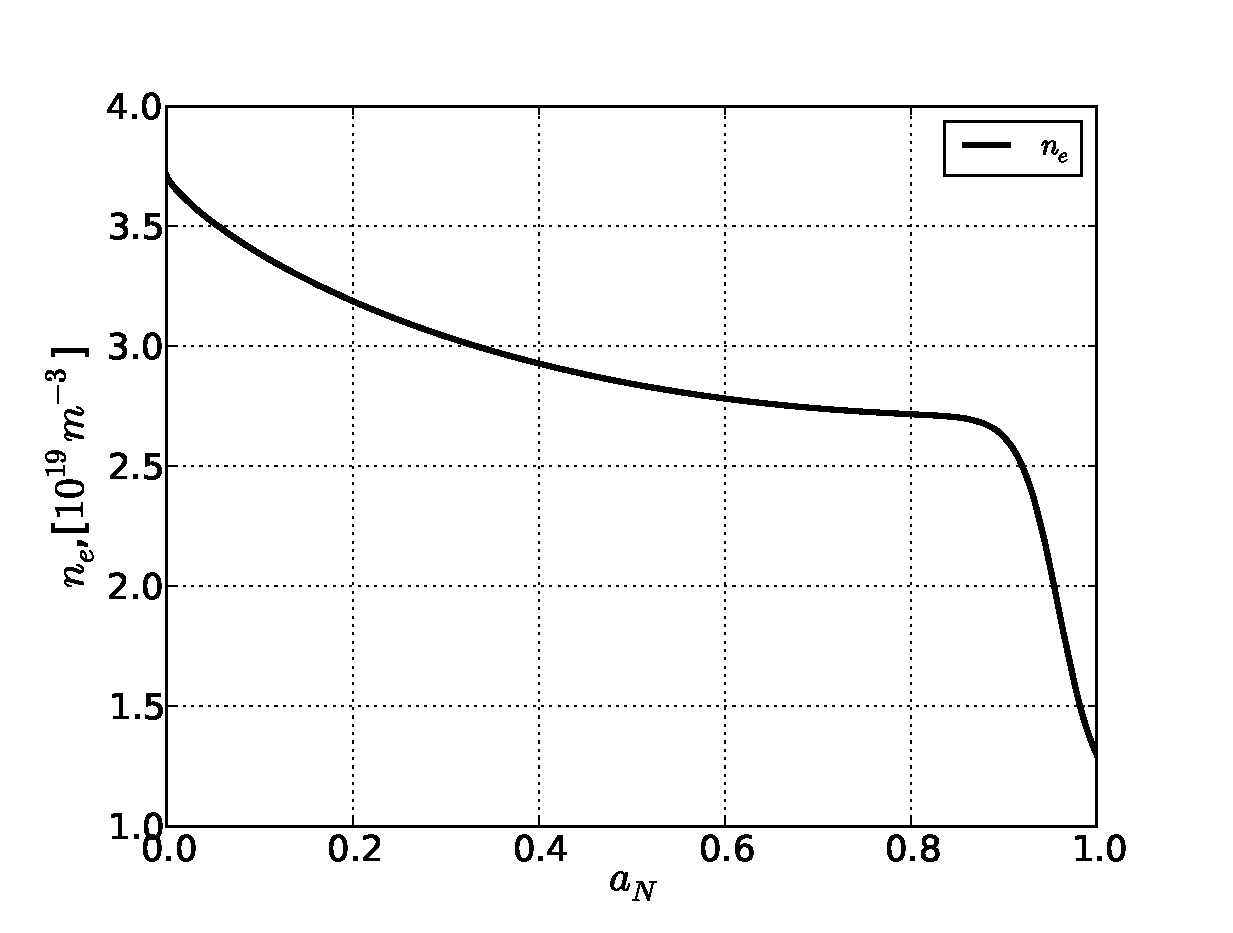
\includegraphics[width=1.35\linewidth]{evans60/ne60.eps}
 \caption{Electron density, $10^{19} m^{-3}$ (NF2013)}
 \label{fig:ne60}
\end{minipage}
\hfill
\begin{minipage}[h]{0.4\linewidth}
 \centering
 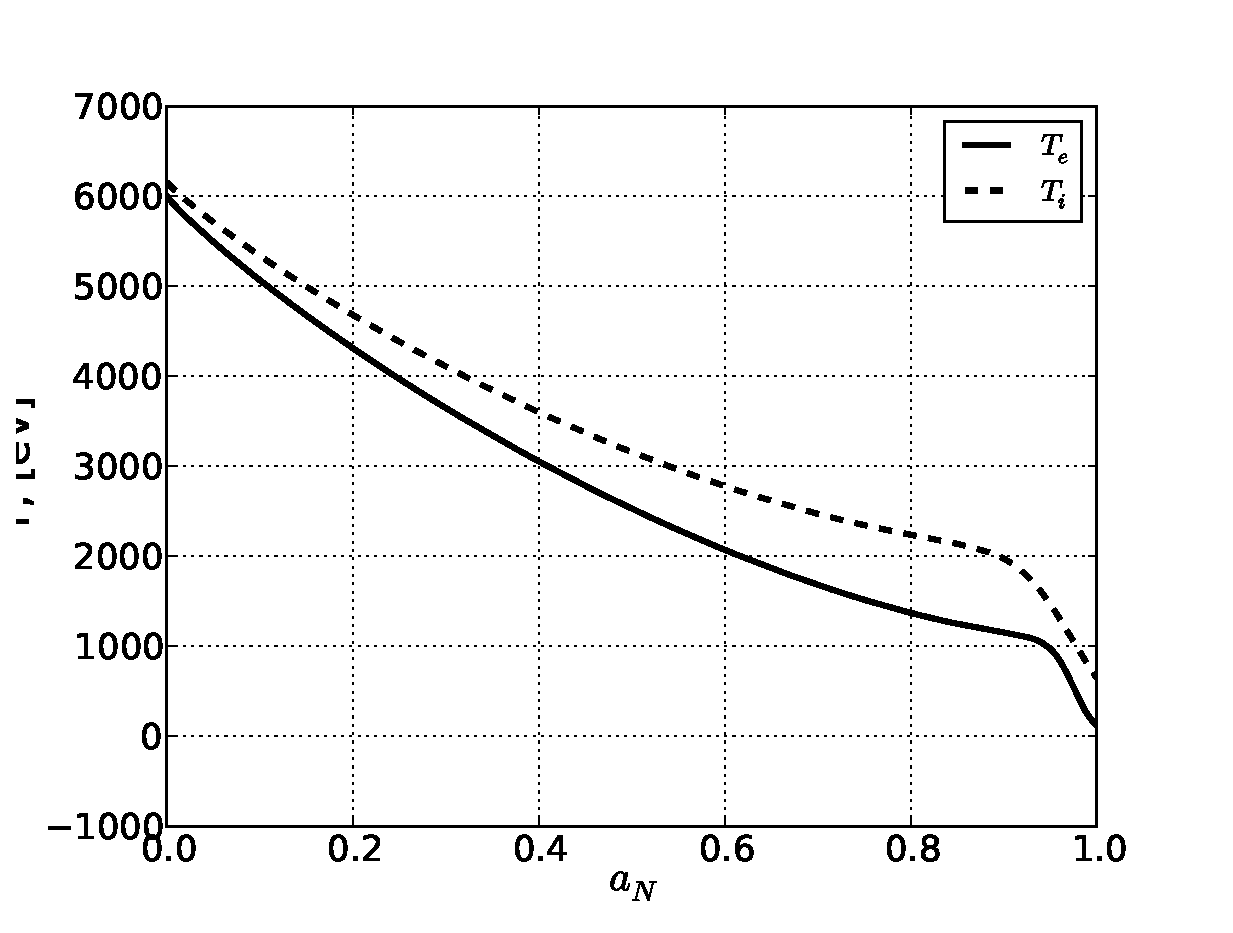
\includegraphics[width=1.35\linewidth]{evans60/T60.eps}
 \caption{Electron and ion temperature, eV (NF2013)}
 \label{fig:T60}
\end{minipage}
\end{center}
\end{figure}
%\newpage
\section{Plasma pressure and pressure gradients}
\begin{figure}[h]
\begin{center}
\begin{minipage}[ht]{0.4\linewidth} 
 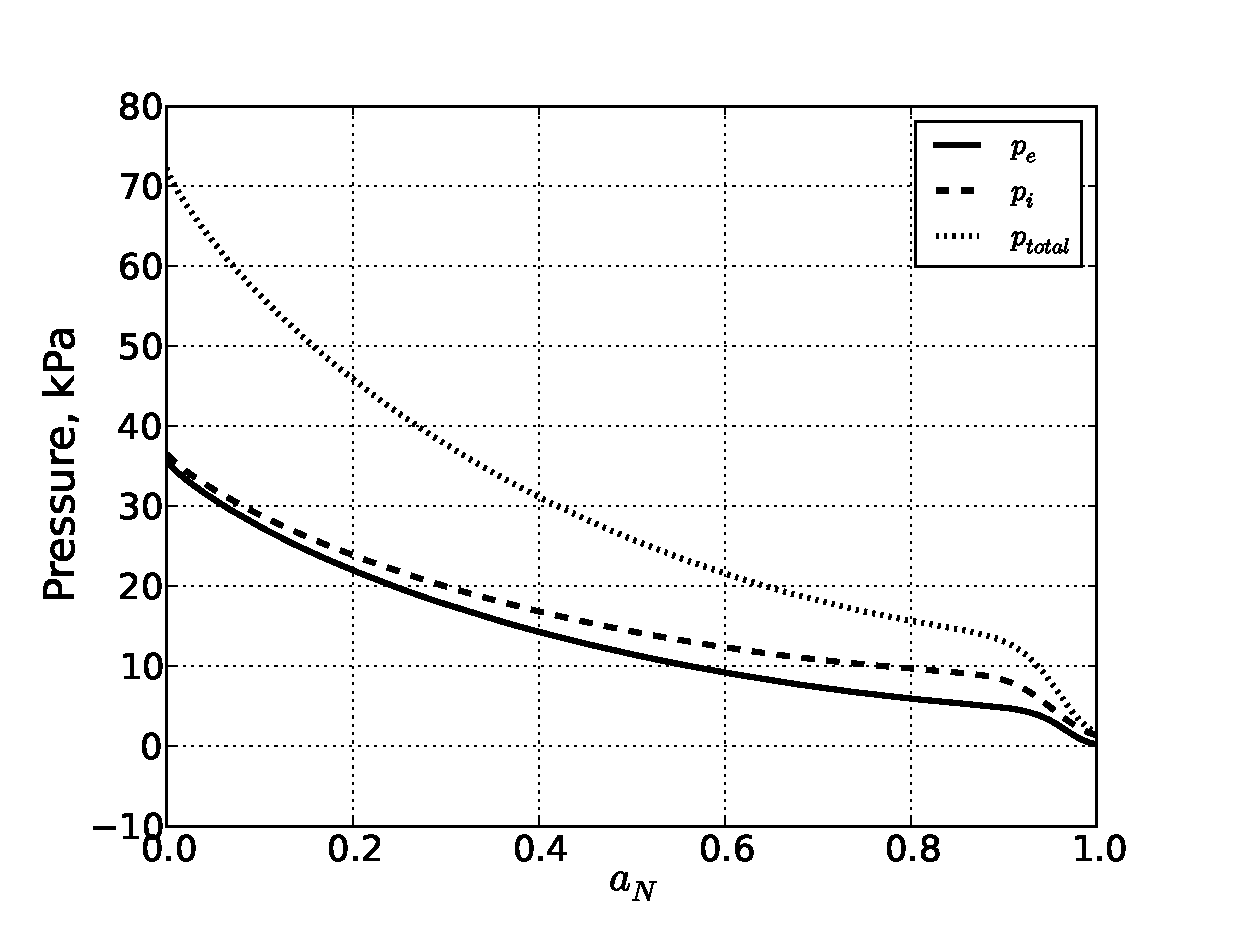
\includegraphics[width=1.35\linewidth]{evans60/P60.eps}
 \caption{Electron, ion and total pressure, $kPa$ (NF2013)}
 \label{fig:P60}
\end{minipage}
\hfill
\begin{minipage}[ht]{0.4\linewidth} 
 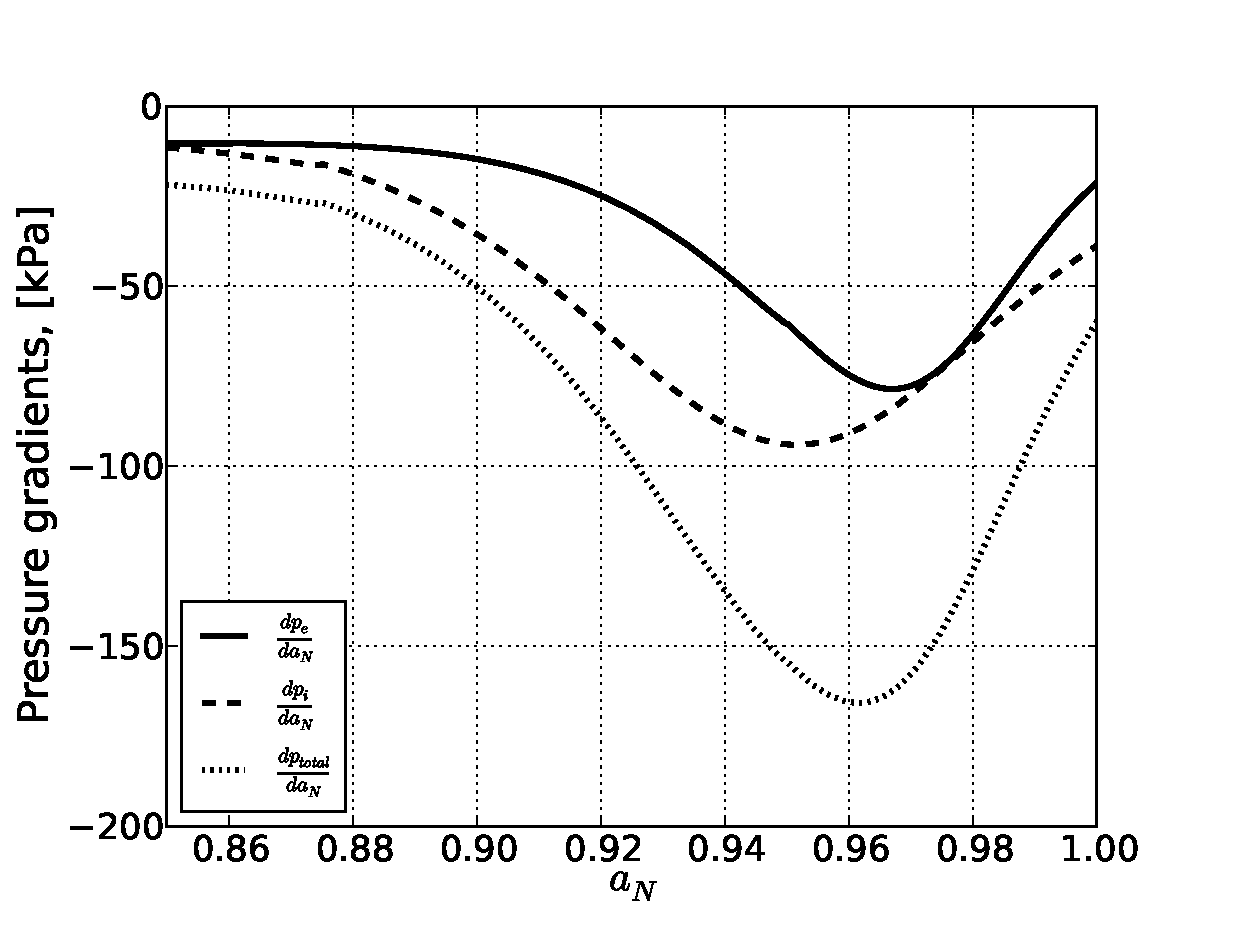
\includegraphics[width=1.35\linewidth]{evans60/dP60.eps}
 \caption{Pressure gradients, $kPa$ (NF2013)}
 \label{fig:DP60}
\end{minipage}
\end{center}
\end{figure}
\newpage
\section{Radial electric field $E_{0r}(a_N)$}
\begin{figure}[ht]
 \centering
 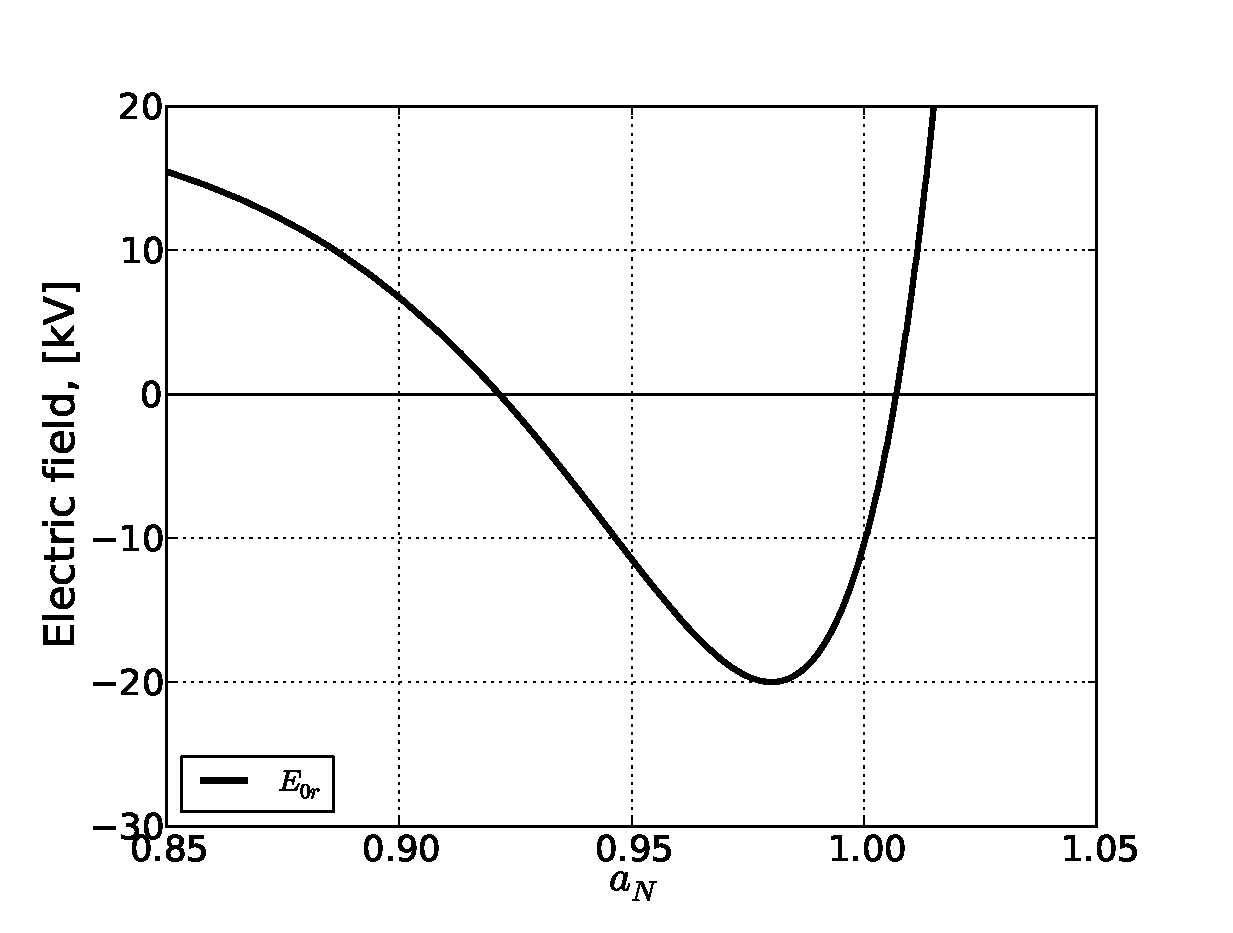
\includegraphics[width=0.55\textwidth]{evans60/E60.eps}
 \caption{Radial electric field, $kV$ (NF2013)}
 \label{fig:Efield60}
\end{figure}
%\newpage
\section{$K_m(a_N)$, $A(a_N)$}
\begin{figure}[h]
\begin{center}
 \begin{minipage}[h]{0.4\linewidth}
  \includegraphics[width=1.35\linewidth]{evans60/K60.eps}
  \caption{$K_m(a_N)$ (NF2013)}
  \label{fig:km60}
 \end{minipage}
 \hfill
 \begin{minipage}[h]{0.4\linewidth}
  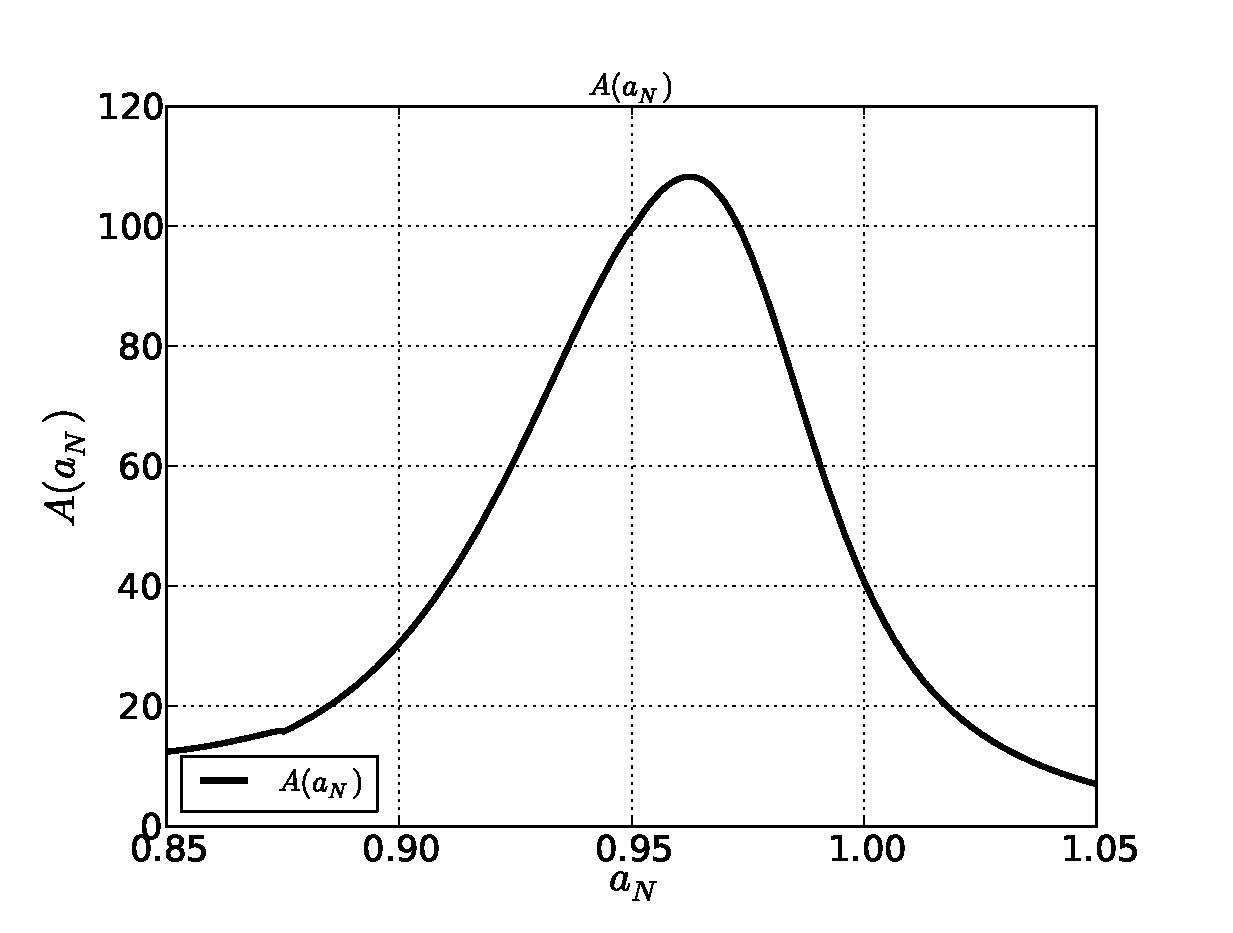
\includegraphics[width=1.35\linewidth]{evans60/A60.eps}
  \caption{$A(a_N)$ (NF2013)}
  \label{fig:A60}
 \end{minipage}  
\end{center}
\end{figure}
\newpage
\section{$Q_m(a_N)$, $Q_{1m}(a_N)$}
\begin{figure}[h]
\begin{center}
\begin{minipage}[h]{0.4\linewidth}
 \includegraphics[width=1.4\linewidth]{evans60/Q60.eps}
 \caption{$Q(a_N):~m=-11,V_{0}=0km/sec$ (NF2013)}
 \label{fig:Q60}
\end{minipage}
\hfill
\begin{minipage}[h]{0.4\linewidth}
 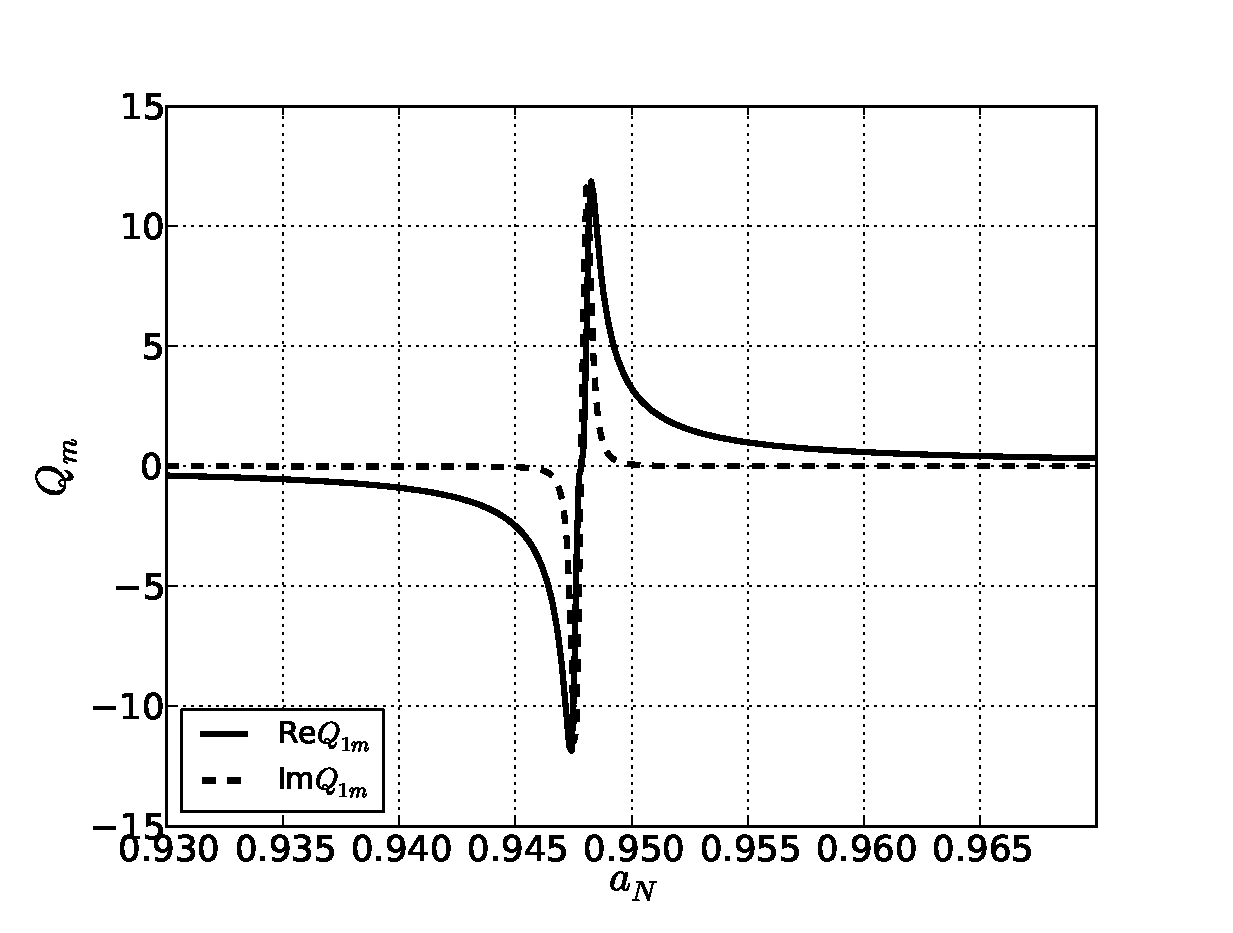
\includegraphics[width=1.4\linewidth]{evans60/Q1_60.eps}
 \caption{$Q_{1m}:~m=-11,V_{0}=0km/sec$ (NF2013)}
 \label{fig:Q160}
\end{minipage}
\end{center}
\end{figure}
\section{Plasma pressure perturbation $P_m$}
\begin{figure}[h]
 \centering
 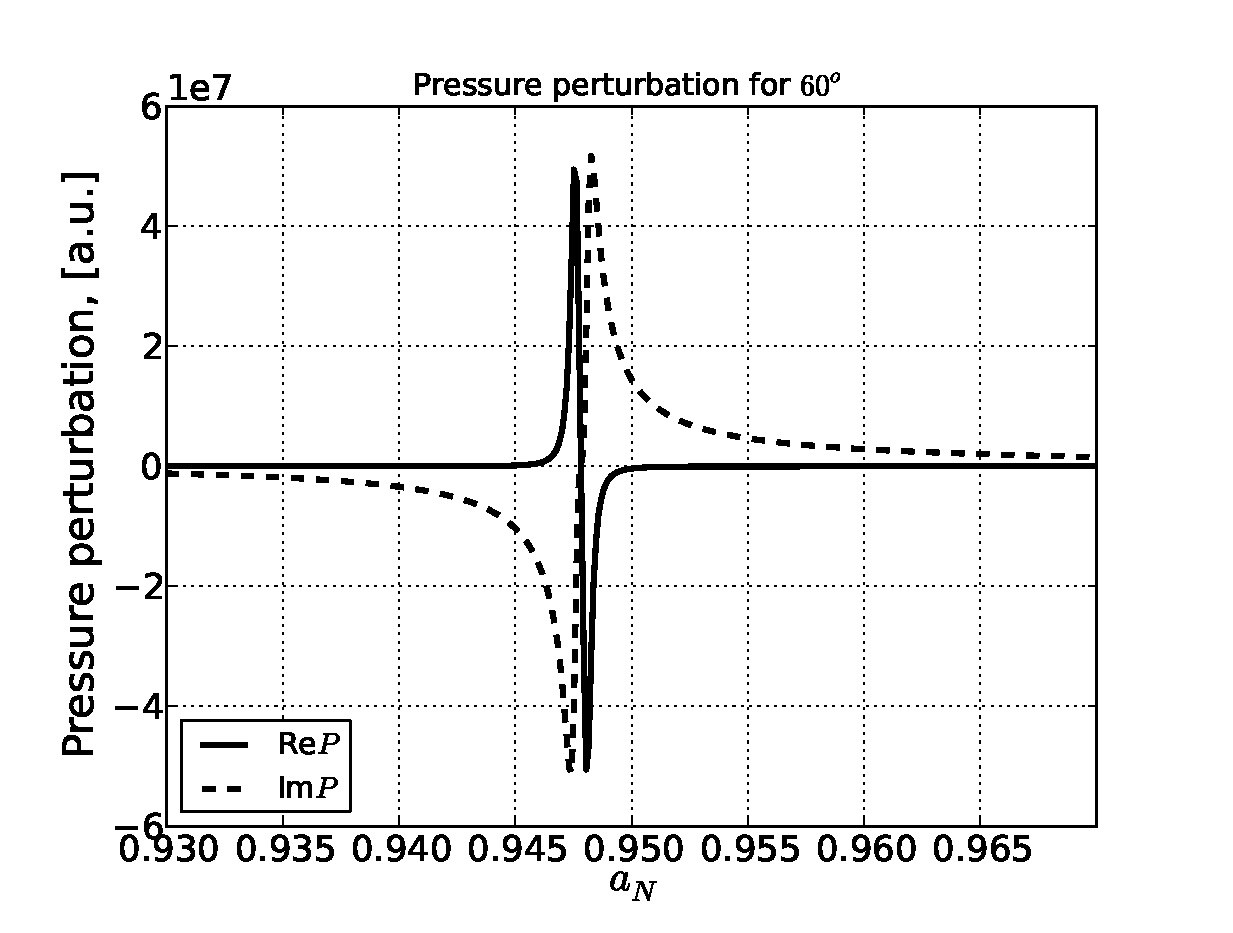
\includegraphics[width=0.7\textwidth]{evans60/perturbation_60.eps}
 \caption{Plasma pressure perturbation (NF2013)}
 \label{fig:pert60}
\end{figure}
\newpage
\part{Bootstrap current}
In progress .................
\end{document}
